\newpage
\section{Model-To-Tree with TGGs}
\genHeader

For those who have read Part IV, do you remember what one of the goals of using TGGs was? We hoped that, by specifying one direction of the transformation, we
could get the other free. That is exactly what's happeded here! The final output of the forward transformation was the model specified in
\texttt{tree.xmi\_fwd.xmi}. This was used as input in the reverse transformation, whose final tree output is \texttt{tree.xmi\_FWD.xmi\_BWD.xmi}. If our
bidirectional transformation was successful, this tree should match the original text instance, \texttt{tree.xmi}. Let's compare the two.

\vspace{0.5cm}

\begin{figure}[htpb]
\begin{center}
  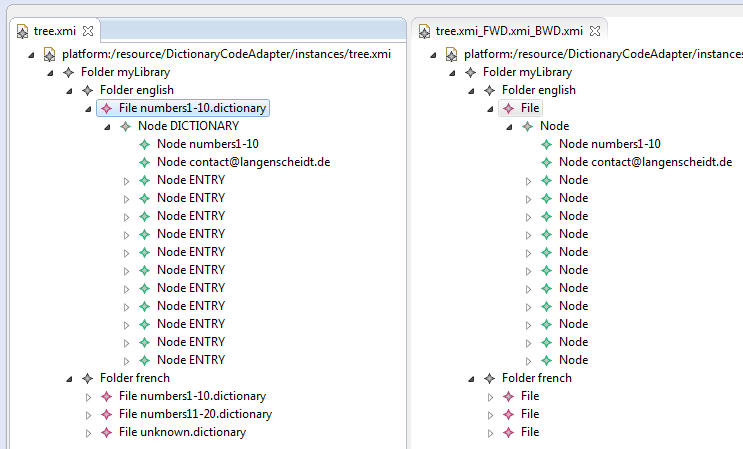
\includegraphics[width=\textwidth]{eclipse_generatedBackwardsModel}
  \caption{needs refinement\ldots}
  \label{eclipse:generatedBkwrdMdl}
\end{center}
\end{figure}

\vspace{0.5cm}

It's close, but not perfect. You can see that some things need to be refined. The ``DICTIONARY'' and ``ENTRY'' labels, for example, are missing from the
major nodes. Luckily, this is a very simple fix. We just need some more attribute constraints!

\jumpDual{m2tvis}{m2ttex}

\newpage
\hypertarget{m2tvis}{}
\subsection{Double-checking the TGG}
\visHeader

\begin{itemize}

\item[$\blacktriangleright$] Open \texttt{NodeToDictionaryRule} and update as depicted below (via attribute constraint). Is this in the right place? Should this
be done before??

\begin{figure}[htp]
\begin{center}
  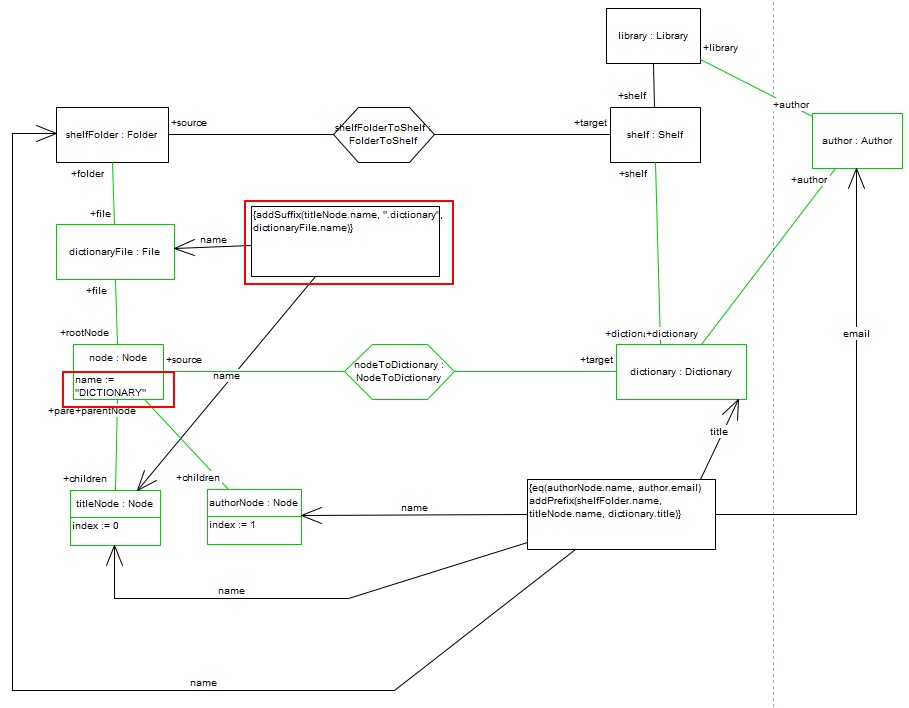
\includegraphics[width=\textwidth]{ea_updateNodeToDictionary}
  \caption{updated NodeToDictionary}
  \label{ea:NodeToDictionary_updated}
\end{center}
\end{figure}

\item[$\blacktriangleright$] Similarly, open \texttt{ForAllEntry} in EA and update like so:

\begin{figure}[htp]
\begin{center}
  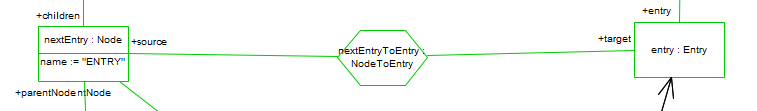
\includegraphics[width=\textwidth]{ea_updateForAllEntry}
  \caption{updated ForAllEntry}
  \label{ea:ForAllEntry_updated}
\end{center}
\end{figure}

\item[$\blacktriangleright$] End comment.

\jumpSingle{finalStep}

\end{itemize}


\newpage
\hypertarget{m2ttex}{}
\subsection{Refining the TGG Transformation}
\texHeader

\begin{itemize}

\item[$\blacktriangleright$] Find the relevant files and add the following attribute constraints. Note : the MOSL parser requires that all attribute constraints
are declared before link variables.

\begin{figure}[htp]
\begin{center}
  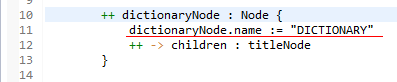
\includegraphics[width=0.8\textwidth]{eclipse_NodeToDictionaryRule_updated}
  \caption[labelInTOC]{needs refinement\ldots}
  \label{eclipse:generatedBkwrdMdl}
\end{center}
\end{figure}

\begin{figure}[htp]
\begin{center}
  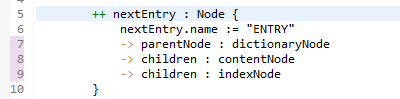
\includegraphics[width=0.8\textwidth]{eclipse_ForAllEntryRule_updated}
  \caption[labelInTOC]{needs refinement\ldots}
  \label{eclipse:generatedBkwrdMdl}
\end{center}
\end{figure} 

\item[$\blacktriangleright$] Add new SetDefaultNumber CSP here.

\begin{figure}[htbp]
\begin{center}
  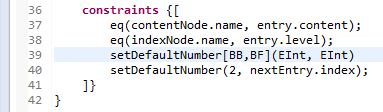
\includegraphics[width=0.6\textwidth]{eclipse_setDefaultNumberConstraint}
  \caption{extra constraint}
  \label{eclipse:newEntryConstraint}
\end{center}
\end{figure}

\end{itemize}

